\documentclass{article}
\usepackage[utf8]{inputenc}
\usepackage{hyperref}
\usepackage{float}
\usepackage{graphicx}
\usepackage{amsmath}
\setlength{\parindent}{0pt}

\title{Intelligent Search and Games: \\ Adantino AI project}
\author{Sam Sweere (6231098)}
\date{October 2019}

\begin{document}

\maketitle

\section{Introduction}
In this report I explain how I made an AI based on a Alpha-Beta search framework on the game of Adantino.

Throughout this project I consciously made decisions to make every function as efficient as I could and encode everything in the smallest size possible. This is done with the intuition that during a search certain functions will be called millions of times, therefore having faster functions will increases the performance of the AI. 

\begin{figure}[ht]
    \centering
    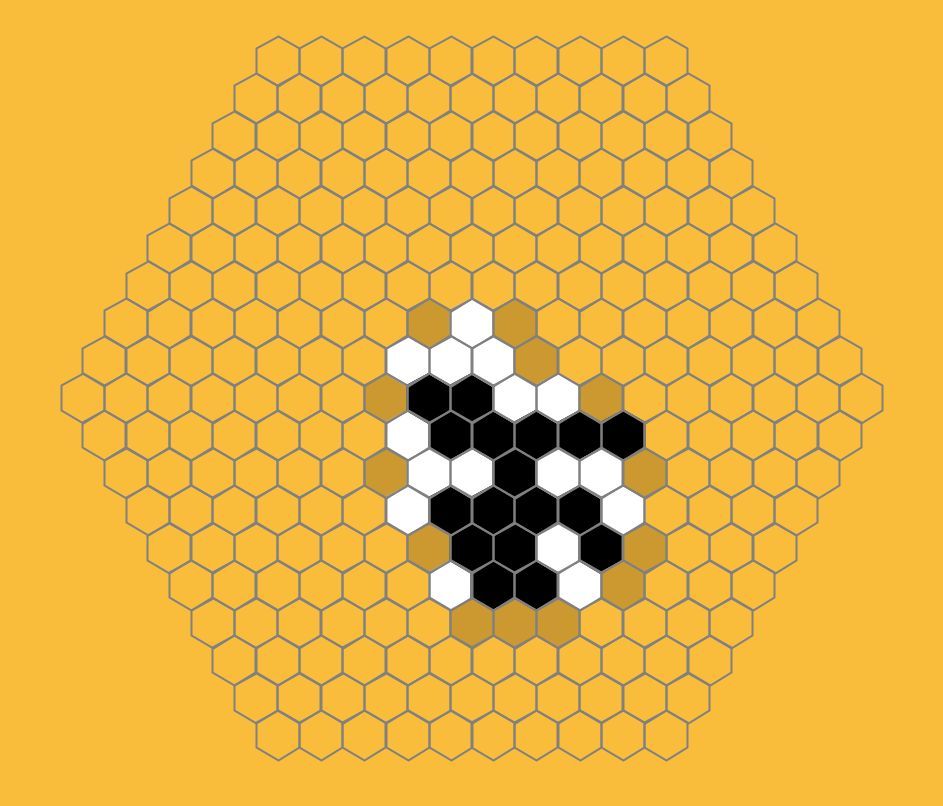
\includegraphics[width = 0.7\textwidth]{images/board.png}
    \caption{An Adantino board}
    \label{fig:board}
\end{figure}

\subsection{The game of Adantino}
\label{sec:adantinoGame}
Adantino is a board game played by two players on a hexagonal board consisting of hexagonal tiles, see figure \ref{fig:board}. The initial board is empty, except the middle tile which is played by the second (black) player. The first (white) player starts, for the first move he can play on any tile directly surrounding the middle (black) tile. After the first move both players can only play on tiles which have at least two neighboring played tiles can be played (dark orange tiles in figure \ref{fig:board}). A player has won if he has 5 tiles in a row or has enclosed the enemy player with his own tiles. For this project the board size that was set to 10 by 10.

\begin{figure}[ht]
    \centering
    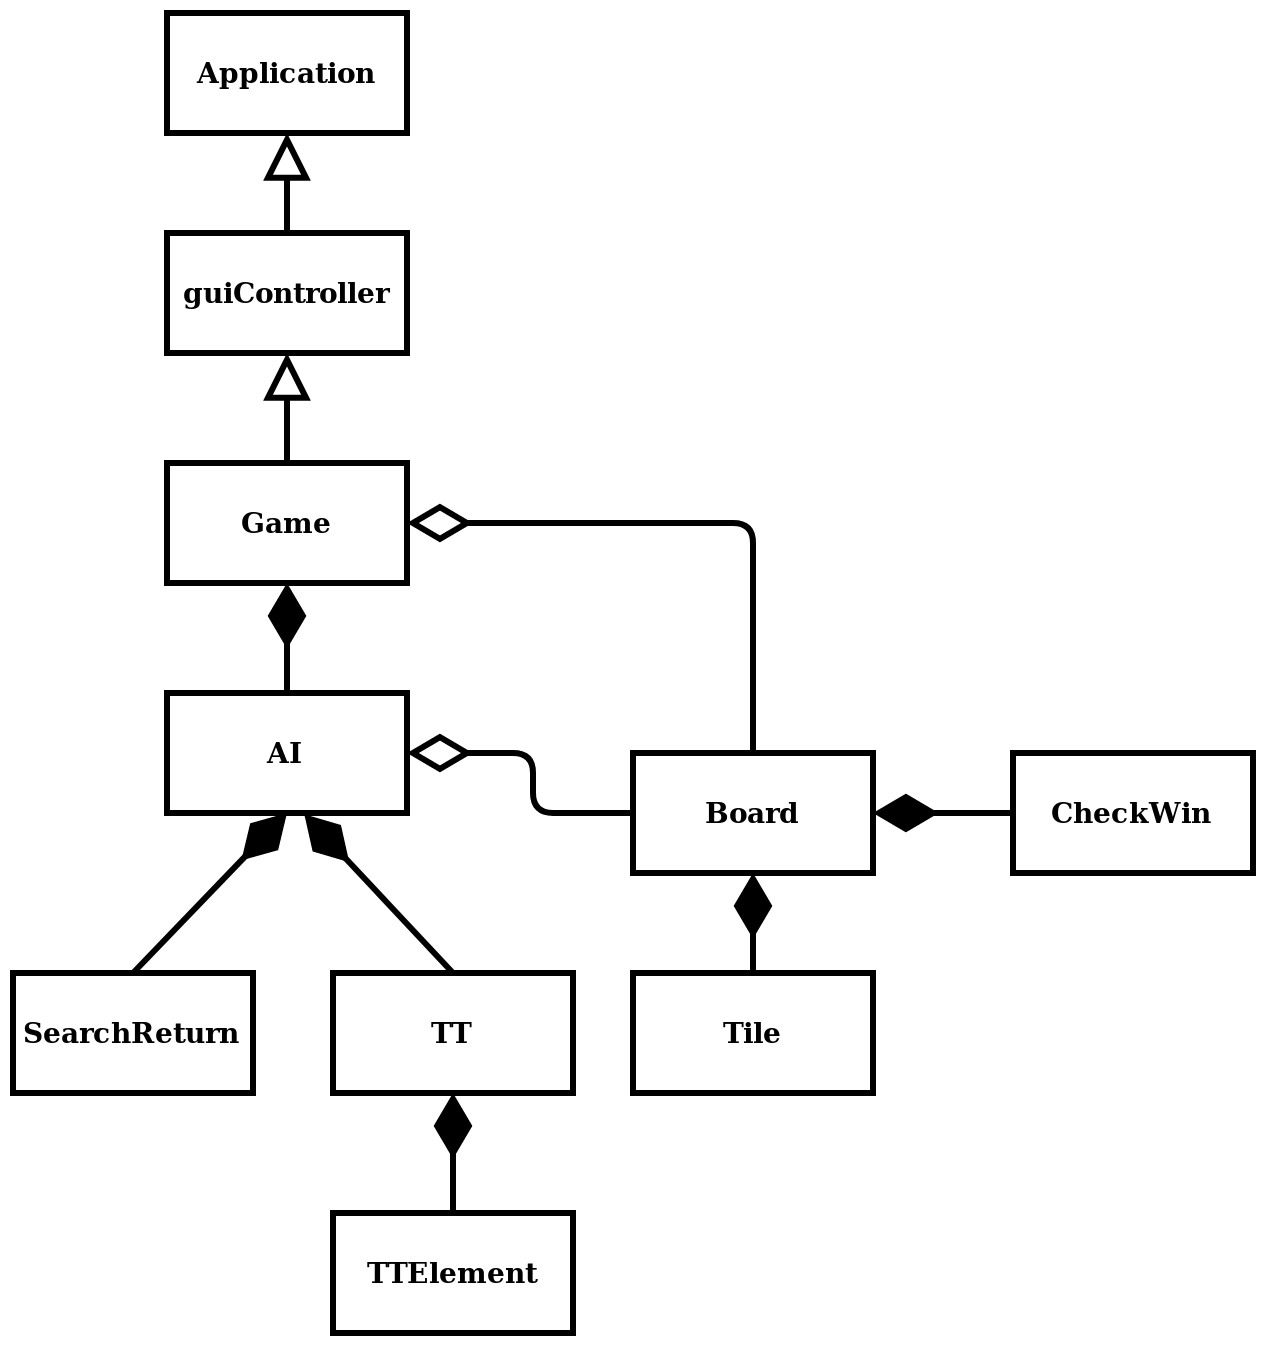
\includegraphics[width = 0.5\textwidth]{images/AdantinoAiUml.png}
    \caption{UML diagram of the Adantino implementation}
    \label{fig:UML}
\end{figure}

\subsection{The program}
I decided to implement the AI in the Java programming language. While I am more comfortable in Python, the performance of the programming language will most likely have as significant influence on the performance of the AI and Java is usually faster than Python. Also this was a excellent opportunity to refine my Java and object-oriented programming skills.
In figure \ref{fig:UML} the UML diagram of the program is visible, during this report I will explain every part of the program, what it does and why I chose to implement it this way.

\section{Implementation of the game}
In this section I will explain how I implemented the game that is playable using a graphical user interface. In later sections I will explain how I created the AI. 

\begin{figure}
    \centering
    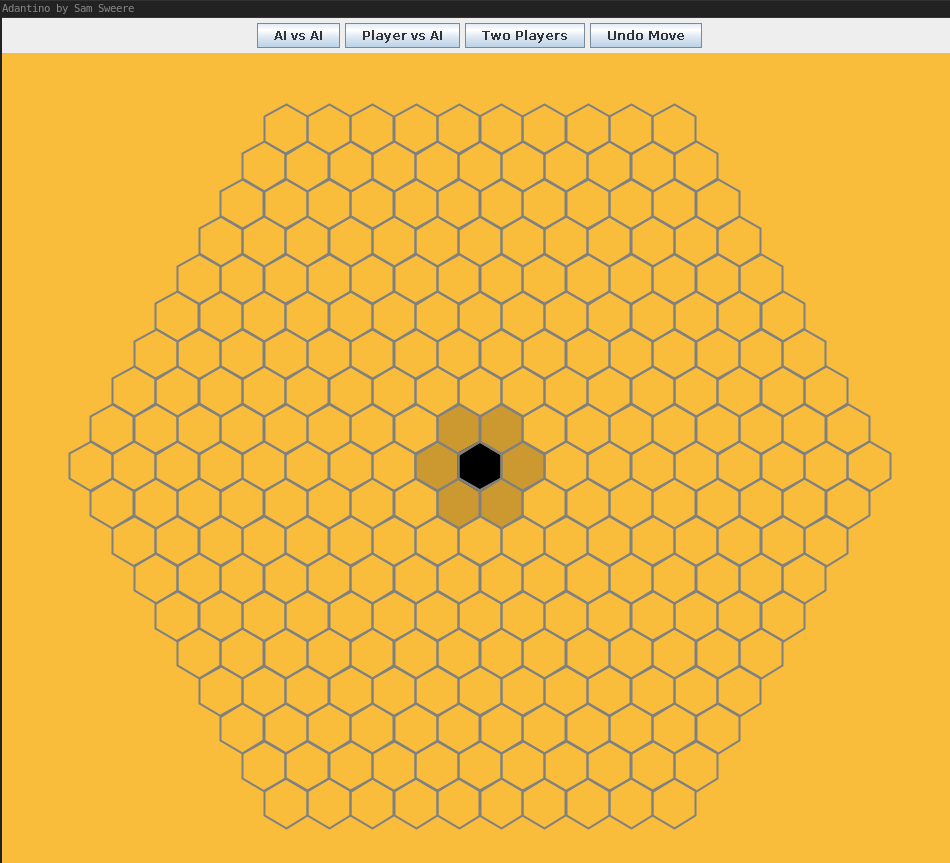
\includegraphics[width = 0.7\textwidth]{images/gui.png}
    \caption{The Adantino graphical user interface}
    \label{fig:gui}
\end{figure}

\subsection{Graphical user interface}
Since Adantino is a board game it is preferable to have a visual board to play on. Therefore I decided to first work on a playable graphical user interface before working on the AI. In figure \ref{fig:gui} the graphical user interface is visible. It consists out of two parts, the board and the menu options. The menu options show the three game-modes: AI vs AI, Player vs AI and Player vs Player. When Player vs AI is requested a popup will ask as what color the human player wants to start. After the human has decided what kind of game it wants to play or see the \textit{guiController} will create this game. The menu options also contains a button for undoing the last human played move.

\begin{figure}[ht]
    \centering
    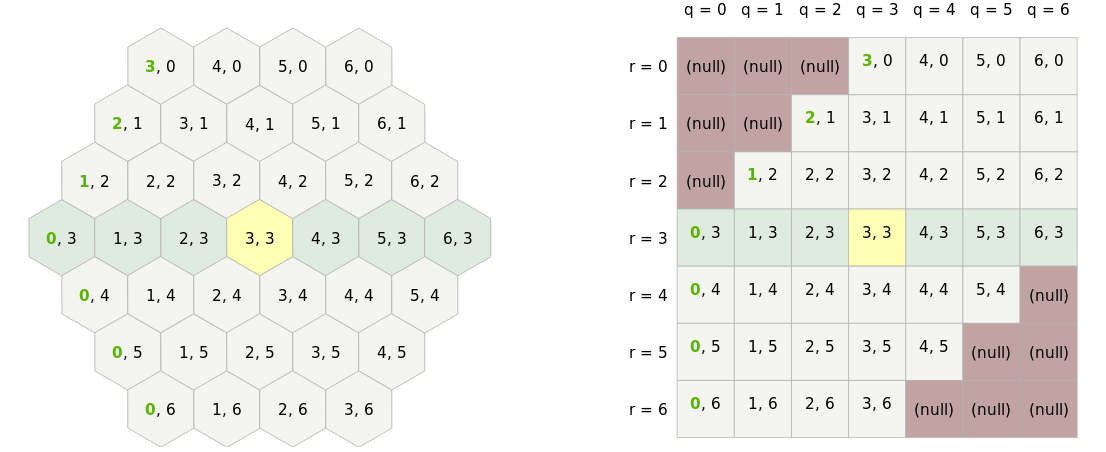
\includegraphics[width = \textwidth]{images/axial-System.png}
    \caption{Axial coordinate system with the array representation, with board radius = 3. Source: \url{https://www.redblobgames.com/grids/hexagons/}}
    \label{fig:axial}
\end{figure}

\subsection{Board Implementation}
The first challenge I encountered when starting to work on this project is on the board layout of Adantino. It consists of hexagonal tiles, a normal coordinate system would not work. After some experimentation and the realisation that making a coordinate system for a hexagon grid was not trivial I started researching online what a good implementation would be. A blog-post of Red Blob Games\footnote{\url{https://www.redblobgames.com/grids/hexagons/}} gave a good overview and I decided to implement it using an axial coordinate system, since this was the most intuitive way for me to work with, while also being space efficient when having to save the board. I programmed the Adantino board such that the board size could be altered, debugging on smaller boards was more convenient. The size is determined by the board radius, that is the distance from the middle tile. The board can then be saved in a two dimensional array with dimensions $(boardRadius*2+1)^2$, see figure \ref{fig:axial}.  

The tiles of the board are saved in a separate Tile class (see figure \ref{fig:UML}). This consists out of four variables:
\begin{itemize}
    \item q: the q (column) value of the tile.
    \item r: the r (row) value of the tile.
    \item s: the state value of the tile, this can be:
    \begin{itemize}
        \item 1: white player played here, displayed as a white tile.
        \item -1: black player played here, displayed as a black tile.
        \item 0: not yet played, displayed as the background color.
        \item 2: not yet played but black will lose if he plays here.
        \item -2: not yet played but white will lose if he plays here.
        \item other values are used during the flood-fill process when checking for win conditions. These will however not propagate out of the checkBoard class.
    \end{itemize}
    \item playable: a boolean that notifies if this tile is playable, displayed as a darker tint of the background color.
\end{itemize}

All these values are stored as bytes to save memory space, the byte number range is from -128 to 127 which is plenty for our implementation. See figure \ref{fig:board} on how such a board looks like.

\subsection{Win conditions implementation}
As explained in section \ref{sec:adantinoGame} in the game of Adantino you can win by either getting 5 tiles in a row or surrounding a tile of the opponent. One way to implement this is to scan the whole board after every move, and check if one of these conditions holds. However, this would be quite inefficient. An observation I made is that the last played tile is always involved in the win condition if there is one. Therefore we only have to check the win conditions starting from the last played tile.  

\subsubsection{5 in a row win condition}
Implementing the 5 in a row win condition was quite easy. From the last played tile we look in all three axis directions with a maximum distance of 4 from the last played tile. If there are 5 tiles in a row in any of these directions the player that made the last move wins.

\subsection{Enclose win condition}
Initially I wanted to implement this win condition by starting at the last played tile and check if by following neighboring tiles of the same colour we are able to enclose the opponent. This could be done by using some kind of shortest path algorithm. However, while thinking about how to actually do this, I encountered a lot of edge cases. For example, how do you do this when you enclose two tiles at the same time but only one of them has a tile of the opponent in it? After a bit of experimentation I came up with a different method that was easier to implement. This method uses a stack based flood fill algorithm starting at every neighboring tile of the last played move that is not of the same player as the last played move. The flood fill algorithm will check every neighboring tile, if the tile is not of the last played player and it has not yet been at this tile it adds this tile to the stack. After it has done this for all its neighbors it marks the tile as visited and takes a new tile from the stack. During this process I also track if we encountered a tile of the opponent. If the stack is empty we know that this area is surrounded by the player. If in this area the opponent was encountered the player (that made the last move) wins. If we did not encounter an opponent in this area we mark these tiles with "the other player loses immediately if he plays here". Because if a player plays in an already surrounded area (for example when the board is almost full and the player has no choice) we do not have do a flood fill again, since we already know this area is surrounded. This also solved the problem of having to do a different kind of flood fill for when a player puts his tile in an already surrounded area.
One other possibility during the flood fill could be that the flood fill ends up at an edge tile. If this is the case we know that we did not enclose the opponent and that it is impossible to do so from this field, we can thus stop the flood fill immediately. This observation led to the choice of using a stack based flood fill approach instead of a queu based. The reason for stack based is that as long as it does not encounter anything it will first search in one direction (depth-first) and thus hit the possible edge of the board faster. Because it hits the possible edge (where we stop the flood-fill immediately) of the board faster it will look at less tiles and is thus more efficient in these scenarios.  
After a flood-fill in one direction is stopped by hitting the edge of the board, we go back and "paint" each previously visited tile. Such that when one of these tiles is visited again in the future when doing a flood fill from a different direction we know that this tile is part of a field that will hit the edge of the board at some point and therefore is not part of an enclosed field, we can thum imediately stop this flood fill.

In the original Adantino rules the board is indefinitely large. The flood fill approach would not work since we would never hit the edge. One solution while still using this flood fill algorithm could be to start of with a small board and make the board dynamically bigger when a tile is played further away from the center. The flood fill would get slower further on in the game but would still work.

%\section{Test setup}
%TODO:
%Not trivial since every implementation is a bit different

%Test on itself:
%Sometimes set depth
%- automaticaly saving depth, sec and nodes

%Maximum test time per ai is 60 seconds. If less last results not saved

%Used a deterministic pseudorandom number genator such that the test would be the same every time.

\section{Alpha-Beta search implementation}
I first implemented a basic recursive Alpha-Beta algorithm in a MiniMax way. This is because it was easier for me to understand what the search is doing when having the Min and Max players, which is useful for debugging. After the basic Alpha-Beta algorithm was in working order I converted it to NegaMax. This makes it easier to add features later on. The basic NegaMax implementation is similar to the one given in the lecture. Therefore I will not explain the workings of Alpha-Beta and NegaMax in this report.

\subsection{Search return}
In order to backpropagate the result of a node I created the SearhReturn class. This class contains the value, the depth where this value was obtained, the principal variation (a list of moves) and a boolean to mark if a search has run out of time.

\subsection{Win and Loss score and windowing}
I defined a win to have the value 100 and a loss to have the value -100. The evaluation function therefore has to generate values between these limits. The reasoning behind these bounds bounds is that the granularity does not become to big. A lot of granularity would decrease the amount of prunes. The value is of course an Integer, otherwise setting these bounds would have been useless. Since the win and loss values are the biggest possible values we can apply a window of $alpha = -100$ and $beta = 100$. Setting the windows increases the amount of pruning and thus increases search performance.

\section{Transposition table and Zobrish hashing}
To increase the performance of the AI I decided to implement a transposition table. Instead of using an off the shelf hash function I decided to implement Zobrish hashing myself. Since Zobrish hashing only uses XOR it is commutative and associative. This means we only have to update the hash after every move for the new board, instead of having to calculate a new hash for the whole board. This again increases performance.

\subsection{Transposition table implementation}
In the transposition table I store the class \textit{TTElement} (see figure \ref{fig:UML}). This consists out of the primary hash, search value, depth, flag and best move. The primary hash is stored as a long and the other as bytes to minimize the space needed for the transposition table. 

Before starting the Alpha-Beta search I first calculate the hash of the whole board, this is then passed on as a parameter during the search. At every move first it is checked if this board is already in the tt. If so we do the same steps as in the lectures. When exploring a new move the hash is updated and passed on.
If an collision occurs I always replace (replacement scheme new).

\subsection{Zobrist hashing implementation}
First we have to decide how many bits our hash should be. Lets make a crude approximation to decide this. Suppose 10 minutes (600 seconds) of calculation time (the maximum time for the AI) and 60000 explored positions per second. This is based on the performance of implementation without tt and assuming no tt hits, this is very pessimistic. In this case the number of positions being mapped is: 
\begin{equation*}
    M = 600*60000 = 3.6*10^{7}
\end{equation*}
We can calculate the probability of an error using:
\begin{equation*}
    P = 1 - e^{\frac{-M^2}{2*2^n}}
\end{equation*}
Lets say we want the chance of an error occurring to be $< 0.1\%$, remember the calculation of $M$ was very pessimistic. If we solve this for $P = 0.1$ and $M = 3.6*10^{7}$ we get $n \approx 52$. The Java Long datatype is 64-bit and thus close to this value. If we use the full 64-bits for the hash this would give us a error probability of $P \approx -3.5*10^{-6}$, well within our margin.

I decided to use 3 bytes (24 bits) as the hash key. Since my memory is sufficiently large why not make use of it, this will also reduce the amount of collisions.

In order to split the hash code (saved as Long) into the primary and secondary hash, I first convert it to a byte array using bit-shifting. Next I use this byte array to take the primary and secondary hash, which are then converted back to Long's using bit-shifting. The reason I use bit-shifting is that it is done in $O(1)$ time complexity. 

\subsubsection{Generating the Zobrist random numbers}
Initially I chose to generate a random number for every possible q (column) value, r (row) value and state. For every tile these three could be combined to create a unique hash for that tile. However, for some reason this caused a lot of collisions. For approximately every 10000 nodes visited there where 5000 collisions. Although we expect some collisions, 50 percent is a bit excessive. I assume this is because having a random number for only the columns and rows is not a smart idea. Since if you do the XOR operation $q XOR q = 0$ (its own inverse) when adding another tile with the same q value it eliminates the q altogether from the hash.    

To solve this problem I changed it to a random value for every unique tile and state, this reduced the amount of collisions to around 6 percent, still quite high but better than 50 percent. I do not know if it is normal to have this many collisions.

\section{Iterative deepening}
To fully make use of the time we have per move I implemented iterative deepening. This starts on depth 1, when it is done searching on this depth and is not out of time it repeats the search process at depth+1. To make use of the values found on the previous search I make use of move reordering using the tt table.

\subsection{Fast wins, slow losses}
During testing I observed that if the AI could win in one move he would not always do this. But rather keep playing knowing that it will win, somewhat taunting the other player. In a similar way the AI would not stop an immediate loss when concluded that it will lose anyway. This makes sense because Alpha-Beta search does not result in the fastest win if it knows it will win. Similarly, when it knows it will lose Alpha-Beta fails in finding good moves. \\
\\
I solved this problem by stopping the iterative deepening the moment a definite win was detected. Since we will win anyway why search deeper? Also this will ensure that the AI will play the fastest win possible: If there is a win in one move it will stop searching at depth 1 and play that move.

When the search results in a definite loss I hope that the opponent has not yet noticed this and we will continue on the depth where the definite loss has not yet been detected. However, if this depth is smaller than two will will not do this, since it cannot detect immediate losses on a depth smaller than two. In addition before starting the Alpha-Beta search I first check if there is an immediate loss if we make a wrong move (loss in two), if so play the move that would block that if possible. This can be done very fast and will save time, since this is an obvious move we do not have to search to higher depths as would otherwise happen. 


%\subsection{The bug}
%This previous method worked for a while, until out of nowhere I started noticing a bug where it will say it will win on depth n, but not win on depth n+1. There are also cases where search will result in a definite win but after the opponent plays one move it will not find a definite win anymore. I spend more then 6 hours debugging to find this problem but was unable to succeed. I have ruled out move ordering, tt and the evaluation function. The only thing it could be is a mistake in how I formulated the win condition or how I do Alpha-Beta search. However, I could not find anything wrong in this by cross referencing the code and looking a log files of how the code was performing on shallow tries. The bug is not game-braking since the AI will still play good moves and is able to beat the AI of other students. This bug could be my Achilles heel during the competition. 

\subsection{Other solutions to the win fast, lose slow}
%Since this bug will give inconsistent definite win or loss conclusions, the previously described method to win fast or lose slow does not work. 
Another solution to the win fast, lose slow problem I tried is by adding the depth, of the win and loss, to the win and loss value. Prioritizing fast wins and slow losses. However, when testing this it decreased the performance quite a bit and it would consistently lose to the AI without this adaptation. This can be explained by that the amount of pruning is reduced when there are multiple win and loss scores. If we take the win and loss value without the depth and we encounter such a win or loss state the search starts to prune a lot of branches. However, when the depth is included in the win and loss scores this pruning can be done to a lesser extend since there are multiple values. Also the alpha part of the window has to be set to the loss value + the maximum search depth, making this part of the window less effective.

%This can be explained in two ways. One is the bug in my program where it would not always conclude it is going to win or lose right. The other explanation could be that the amount of pruning is reduced when there are multiple win and loss scores. Without taking the depth into account when the search encounters a win or loss it can start pruning a lot of nodes. However when the win and loss scores can be multiple values this pruning can be done to a lesser extend. Also the alpha part of the window has to be set to the loss value + the maximum search depth, making this part of the window less effective.\\
%\\
%Since this was not going to work I decided to implement a weaker solution. Before starting the Alpha-Beta search I first check if there is a win in one move, if so play that, and if there is a loss in two move, if so block that if possible. These can be done very fast and will save time where an obvious move can be made.

\subsection{Out of time}
For every search the is a maximum time, when this max search time is reached we have to stop. When during the search process we explore a new node we first check if we are still within the max time limit. If not we set the out of time boolean in the search return to true and return this. When the root receives a search return were the out of time boolean is true it knows that the search was not completed and takes the best move from the principal variation of the previous iterations (depth - 1). 

\section{Evaluation function}
When during the search a leaf node arrives at a board where none of the win condition are met we can still give a score to this board. This score is based on heuristics and calculated using an evaluation function. In my implementation the evaluation function has to return an Integer value between -99 and 99 (since -100 and 100 are for win conditions) where the positive number is in advantage of the white player. Also the -1*value should be the evaluation score for the opponent. For this AI I developed two evaluation functions based on the group size and number of neighbours.

\subsection{Evaluation function based on group size}
This evaluation function is based on the heuristic that having a lot of connected tiles as a player is good. Since having a lot of connected tiles increases the options to get a win condition for 5 in a row or an enclose. The score is based on how many tiles are in the field of a tile. Thus if white has two connected tiles the score is $2+2=4$ and three connected tiles $3+3+3=9$. This heuristic of course also holds for the oponent player and blocking him would be a good idea. Therefore the total score is based on the difference of the two players. However, this value can become bigger than 100, which is not allowed. To solve this instead of taking the score directly we take the relative score and multiply it by 99 (the evaluation score is always in advantage of the white player): 
\begin{equation*}
    evalScore = \left(\frac{whiteScore}{whiteScore+blackScore}-\frac{whiteScore}{whiteScore+blackScore}\right)*99
    \label{eq:relativeScore}
\end{equation*}

I implemented the counting of connected tiles by scanning all the tiles of the board and doing a flood fill from the tile if it belongs to one of the players. The amount of visited tiles of this player during the flood fill will be added to the players score. 

\subsection{Evaluation function based on number of neighbours}
An observation I made when looking at the scores of the evaluation function based on group size is that using this evaluation function greatly reduced the speed at which nodes could be visited, and thus reducing the maximum search depth. Thinking about how this evaluation could be sped up I noticed that the heuristic could also be interpreted in a different way. Instead of a tile being part of a big group we could also look at how many neighbors of the same colour the tile has. Again, having more neighbours increases the options for the win conditions 5 in a row and enclose. Instead of doing a flood fill we now only have to look at the direct neighbors, which increased the speed a lot.

\subsection{Testing the evaluation functions}
To test which evaluation function performs best I first let the AI with no evaluation function play against the AI with the group evaluation function. Both play one game as white and one game as black. The AI's where both using tt and iterative deepening. The maximum time per move was set to 20 seconds, since that approximate the time the AI has during the competition (see section \ref{sec:tpm}). There was no maximum search depth since there is already a time limit and we want the AI to play the best move it can find in this time.

TODO: AI no Evaluation function vs AI groupsize evaluation function

The AI with the groupsize evaluation function won both games from the AI with no evaluation function. 

Next we test if an AI with the neighbours evaluation function will beat an AI with the groupsize evaluation function.

TODO: 


\section{Time per move}
\label{sec:tpm}
For the competition there is a maximum time the AI can take for playing one game, therefore we need a way to determine the maximum time per move. We will use the following equation that determines the maximum time for a move:
\begin{equation*}
    tM(gT, cP, m, cm, gTL pP)= 
\begin{cases}
    \frac{gT*cP}{cm},& \text{if } m\leq cm\\
    gTL*pP,            & \text{otherwise}
\end{cases}
\end{equation*}
Where $tM$ is max time for this move in sec, $gT$ is max game time in sec, $cP$ is percentage for comfortable moves, $m$ is amount of moves already made, $cm$ is amount of comfortable moves, $gTL$ is game time left in sec and $pP$ is panic percentage.
To determine these variables I used the following reasoning:
Most games take around 40 moves total (both sides). Thus pessimistically 50 moves (both sides). This means we should be able to take 25 moves (only AI side) comfortably ($cm = 25$). Of the total game time  10 minutes ($gT = 600 sec$) we take a percentage ($cP = 0.08$) for the comfortable moves. These moves will take $\frac{gT*cP}{cm} = \frac{600*0.8}{25} = 19.2 sec$. If we taken more moves than we comfortably can we go into panic mode. In this mode we take a percentage ($pP = 0.08$) of the remaining time ($gTL$, $gTL \geq gT*(1-cP)$) for each move. This ensures that in panic mode at first we still have some time per move, assuming the game will be over fast, but we will also always make a move, be it in a short calculation time if the game takes longer.  

The max time per move ($tM$) is thus constant for the first $cM$ moves and after that it decreases exponentially.


\iffalse
\section{Learned lessons}
- lesson on signed values, the abs(INTEGER.MIN\_Value) is bigger than the INTEGER.MAX\_Value. Thus when -1*INTEGER.MIN-VALUE it loops around to another small MIN-VALUE.

- Undo function, this function skips to the human turns. Since the AI is deterministic an Undo has no use.


- The alpha beta search needs to start with a move, but for the first row this is a problem. In order to avoid having to make a starting function I defined a move with Max int value to be the start. This skips the winning evaluation and goes to the second part of the alpha beta search.

- Implemented a pv class. Such that the depth can be taken into account when checking. And eventual future extentions can be added. This also eliminates the need for a seperate staring function that checks the best value from root

- Implemented animation by refreshing the pane as an action

- 

- Doing a full refractor of the code later on would have been benificial.

\fi
%\section{Future improvements}
%Include pn-search on second thread;
%Continuasly build tt table on second thread;

\section{Future work}
If I would improve this AI in the future I would start by refactoring the code. When making a program like this in the timespan of multiple weeks it is almost impossible to predict what classes and datastructures would be most practical. Every week when I added a new part I had to go into previously defined function to alter or add variables and/or functions. After a while the readability and ease of adaptation starts to become worse. Refactoring the whole code would solve this problem and make it easier to work on in the future, however it will probably take quite some time. %After the refactoring I will try to find and fix the bug that makes this AI unreliable.
\\
\\
There are quite some improvements that could be made to this AI. One of the easiest to add to this AI would be killer moves and history heuristics. Also the multiple cores of modern cpu's could be utelized. Alpha-Beta search can only be done on one thread on one core, but expanding for example the tt with other Alpha-Beta searches with different move ordering could improve the performance of the main Alpha-Beta search.
\\
\\
Another extension that would be interesting to add would be a proof-number search in a second thread. It would be interesting to see how well proof-number search works on a game such as Adantino.

\end{document}
